\documentclass[9pt,twocolumn,twoside,lineno]{pnas-new}

%% Some pieces required from the pandoc template
\providecommand{\tightlist}{%
  \setlength{\itemsep}{0pt}\setlength{\parskip}{0pt}}

% Use the lineno option to display guide line numbers if required.
% Note that the use of elements such as single-column equations
% may affect the guide line number alignment.


\usepackage[T1]{fontenc}
\usepackage[utf8]{inputenc}



\templatetype{pnasresearcharticle}  % Choose template

\title{A Standardized Effect Size for Evaluating and Comparing the Strength of
Phylogenetic Signal}

\author[a,1]{Dean C. Adams}
\author[a,b]{Erica K. Baken}
\author[b]{Michael L. Collyer}

  \affil[a]{Department of Ecology, Evolution, and Organismal Biology, Iowa State
University, Ames, Iowa, 50010. USA.}
  \affil[b]{Department of Science, Chatham University, Pittsburgh, Pennsylvania,
15232. USA.}


% Please give the surname of the lead author for the running footer
\leadauthor{Adams et al.}

% Please add here a significance statement to explain the relevance of your work
\significancestatement{Evolutionary biologists wish to quantify and compare the strength of
phylogenetic signal across traits, but analytical tools for these
comparisons are generally lacking. Here we develop a standardized effect
size based on \(\kappa\), (\(Z_\kappa\)), which measures the strength of
phylogenetic signal on a common statistical scale, and provides a
mechanism for formally comparing the strength of phylogenetic signal
across datasets. Additionally, we find that a commonly used parameter
(Pagel's \(\lambda\)) is unsuitable for this purpose. Our procedure
enables biologists to quantitatively address hypotheses that compare the
strength of phylogenetic signal between various phenotypic traits, even
when those traits are found in different evolutionary lineages or have
different units or scales.}


\authorcontributions{D.C.A. designed the research; D.C.A., E.K.B., and M.L.C. performed the
research and wrote the paper.}

\authordeclaration{The authors declare no conflict of interest. \hfill\break

Data deposition: Data for the empirical example may be found on DRYAD:
\url{doi:10.5061/dryad.b554m44} and \url{doi:10.5061/dryad.59zw3r23m}.
R-scripts for simulation tests are found on Github: XXX. Computer code
for implementing the two-sample comparison of effect sizes is found in
geomorph:
\url{https://cran.r-project.org/web/packages/geomorph/index.html}
\hfill\break

\textsuperscript{1}To whom correspondence should be addressed. E-mail:
\href{mailto:dcadams@iastate.edu}{\nolinkurl{dcadams@iastate.edu}}}


\correspondingauthor{\textsuperscript{} }

% Keywords are not mandatory, but authors are strongly encouraged to provide them. If provided, please include two to five keywords, separated by the pipe symbol, e.g:
 \keywords{  phylogenetic signal |  macroevolution |  lambda |  kappa  } 

\begin{abstract}
Macroevolutionary studies frequently characterize the phylogenetic
signal in phenotypes, and wish to compare the strength of that signal
across traits. However, analytical tools for such comparisons have
largely remained underdeveloped. Here we evaluate the efficacy of one
commonly used parameter (Pagel's \(\lambda\)) to estimate the strength
of phylogenetic signal in phenotypic traits, and evaluate the degree to
which \(\lambda\) correctly identifies known levels of phylogenetic
signal. We find that \(\lambda\) behaves as a Bernoulli random variable,
and that estimates are increasingly skewed at larger and smaller input
levels of phylogenetic signal. Further, the precision of \(\lambda\) in
estimating actual levels of phylogenetic signal is often inaccurate, and
biological interpretations of the strength of phylogenetic signal based
on \(\lambda\) are therefore compromised. As an alternative, we propose
a standardized effect size based on \(\kappa\), (\(Z_\kappa\)), which
measures the strength of phylogenetic signal more reliably than does
\(\lambda\), and places that signal on a common scale for statistical
comparison. We develop tests based on \(Z_\kappa\) to provide a
mechanism for formally comparing the strength of phylogenetic signal
across datasets, in much the same manner as effect sizes may be used to
summarize patterns in quantitative meta-analysis. Our approach extends
the phylogenetic comparative toolkit to address hypotheses that compare
the strength of phylogenetic signal between various phenotypic traits,
even when those traits are found in different evolutionary lineages or
have different units or scales.
\end{abstract}

\dates{This manuscript was compiled on \today}
\doi{\url{www.pnas.org/cgi/doi/10.1073/pnas.XXXXXXXXXX}}

\begin{document}

% Optional adjustment to line up main text (after abstract) of first page with line numbers, when using both lineno and twocolumn options.
% You should only change this length when you've finalised the article contents.
\verticaladjustment{-2pt}

\maketitle
\thispagestyle{firststyle}
\ifthenelse{\boolean{shortarticle}}{\ifthenelse{\boolean{singlecolumn}}{\abscontentformatted}{\abscontent}}{}

% If your first paragraph (i.e. with the \dropcap) contains a list environment (quote, quotation, theorem, definition, enumerate, itemize...), the line after the list may have some extra indentation. If this is the case, add \parshape=0 to the end of the list environment.

\acknow{We thank E. Glynne and B. Juarez for comments on early drafts of the
manuscript. This work was supported in part by NSF grant DBI-1902511 (to
D.C.A.) and DBI-1902694 (to M.L.C.). \hfill\break}

Investigating macroevolutionary patterns of trait variation requires a
phylogenetic perspective, because the shared ancestry among species
violates the assumption of independence among trait values that is
common for statistical tests (1, 2). Accounting for this evolutionary
non-independence is the purview of \emph{phylogenetic comparative
methods} (PCMs): a suite of analytical tools that condition trends in
the data on the phylogenetic relatedness of observations (3--12). These
methods are predicated on the notion that phylogenetic signal -- the
tendancy for closely related species to display similar trait values --
is present in cross-species datasets (1, 13, 14). Indeed, under numerous
evolutionary models, phylogenetic signal is to be expected, as
stochastic character change along the hierarchical structure of the tree
of life generates trait covaration among related taxa (1, 14, 15).

Several analytical tools have been developed to quantify phylogenetic
signal in phenotypic datasets (13, 14, 16--19), and their statistical
properties -- namely type I error rates and statistical power -- have
been investigated to determine under what conditions phylogenetic signal
can be detected (15, 18, 20--25). One of the most widely used methods
for characterizing phylogenetic signal is Pagel's \(\lambda\) (13),
which transforms the lengths of the internal branches of the phylogeny
to improve the fit of data to the phylogeny via maximum likelihood (13,
26). When incorporated in PGLS, \(\lambda\) serves as a tuning parameter
which is optimized via log-likelihood profiling while evaluating the
covariation between the dependent and independent variables, given the
phylogeny (13, 26). To infer whether phylogenetic signal differs from no
signal or a Brownian motion model of evolutionary divergence, the
observed model fit using \(\hat\lambda\) may be statistically compared
to that using \(\lambda=0\) or \(\lambda=1\) via likelihood ratio tests
(26--28) or confidence limits (29). Another widely used measure is
Blomberg's \(\kappa\) (14), which measures the ratio of observed trait
variation to the amount expected under Brownian motion. Blomberg's
\(\kappa\) can be treated as a test statistic by employing a permutation
test to generate its sampling distribution (14, 18) for determining
whether significant phylogenetic signal is present in data. Both
\(\lambda\) and \(\kappa\) seem intuitive to interpret, as a value of
\(0\) for both corresponds to no phylogenetic signal, while a value of
\(1\) corresponds to the amount of phylogenetic signal expected under
Brownian motion. Thus, it is tempting to regard both \(\lambda\) and
\(\kappa\) as descriptive statistics that measure the relative strength
of phylogenetic signal, providing an estimate of its magnitude for
comparison.

The appeal of Pagel's \(\lambda\) and Blomberg's \(\kappa\) as
descriptive statistics is that they provide a basis for interpreting
``weak'' versus ``strong'' phylogenetic signal; i.e., small versus large
values of \(\hat{\lambda}\) or \(\kappa\), respectively, in a
comparative sense (30--32). Nonetheless, an important question that has
yet to be considered is whether these statistics are or can be converted
to effect sizes for comparative analyses across datasets? To be
statistics representing phylogenetic signal, they should have reliable
distributional properties, which could be revealed with simulation
experiments. For instance, as a proportional random variable bounded by
\(0\) and \(1\), we might expect that \(\hat{\lambda}\) follows a
Bernoulli distribution (\textbf{add ref}); i.e., branch lengths in a
tree are scaled proportionally to the probability that data arise from a
BM process. Given a known \(\lambda\) value used to generate random data
on a tree, we would also expect that the mean of an empirical sampling
distribution of \(\hat{\lambda}\) would approximately equal \(\lambda\);
the dispersion of \(\hat{\lambda}\) would be largest at intermediate
values of \(\lambda\), \(\hat{\lambda}\) would be predictable over the
range of \(\lambda\) with respect to treesize; the distribution of
\(\hat{\lambda}\) would be symmetric at intermediate values of
\(\lambda\) and more skewed toward values of 0 or 1; and that the
distribution of \(\hat{\lambda}\) will be more platykurtic at
intermediate values of \(\lambda\), becoming more leptokurtic toward 0
and 1 (\textbf{add same ref}). Prior work (20) seems to support some of
these conjectures, based superficially on statistical moments for a
given tree size (mean, variance, skewness, and kurtosis; see Fig. 2 of
ref. (20)). However, because the ``strength of Brownian motion'' was
simulated as a varied weighted-average of data simulated on trees with
\(\lambda=0\) and \(\lambda=1\) and not as prescribed values of
\(\lambda\) (20), interpretation of these patterns is challenging.

By contrast, Blomberg's \(\kappa\), which is positively ubounded, might
be expected to follow a normal distribution (\textbf{add ref}). Thus we
might expect that \(\kappa\) is symmetrically distributed across
different strengths of phylogenetic signal, for any \(\lambda\) used to
generate data. This attribute seemed less reasonable based on the
simulations performed by Münkemüller et al.~(20), which suggested that
distributions were positively skewed and that Blomberg's \(\kappa\)
might not behave as a statistic that follows a normal distribution.
However, because their simulations used a weighted combination of
simulated phylogenetic signal strengths, strong inferences are not
possible (and distributional attributes were not the intended result of
their simulations). Thus, for both Pagel's \(\lambda\) or Blomberg's
\(\kappa\), evaluation of statistical moments across a range of
\(\lambda\) used to generate data would be valuable for adjudicating the
relibalilty of these statistics. Furthermore, these are statistics that
appear to have expected values that vary with tree size (20), making
comparisons across studies challenging. Therefore, transformation of
these statistics into \(Z\)-scores in the same simulation experiments
would allow evaluation of the efficacy of each statistic to yield effect
sizes that could be used for comparisons of the strength of phylogenetic
signal across traits and clades.

Here we used simulation experiments to compare the distributional
attributes of \(\hat{\lambda}\) and \(\kappa\), plus their effect sizes
(\(Z\)-scores), across a range of tree size and phylogenetic signal
strength. We find that estimates of \(\hat{\lambda}\) are increasingly
skewed at larger and smaller input levels of phylogenetic signal and at
smaller tree sizes, vary widely for a given input value of \(\lambda\),
and that the precision of \(\hat{\lambda}\) is not constant across its
range. By contrast, estimates of \(\kappa\) are more consistent across
tree sizes, and are normally distributed across the range of input
levels of \(\lambda\), making \(\kappa\) a more reliable statistic. We
then propose an effect size based on \(\kappa\), (\(Z_{\kappa}\)), which
provides consistent estimates of the strength of phylogenetic signal
across tree sizes and signal strength, and facilitates quantitative
comparisons of the relative strength of phylogenetic signal across
datasets.

\hypertarget{results}{%
\section{Results}\label{results}}

\textbf{Lambda (\(\lambda\)) estimates of phylogenetic signal are
innacurate.} Computer simulations revealed that for \(\hat{\lambda}\),
the distributional expectations of a Bernoulli variable were mostly
upheld. First, the mean value of \(\hat{\lambda}\) did increase as
\(\lambda\) increased, but it was negatively-biased (particularly for
small tree sizes), and was consistently less than the input \(\lambda\)
value across most of its range (Fig. 1 black line). Second, the standard
deviation of \(\hat{\lambda}\) was largest at intermediate values of
\(\lambda\) and smallest at extreme values, implying that the precision
in estimating \(\lambda\) varied across the range of input values (Fig.
1 red line). Additionally, standard deviations of \(\hat{\lambda}\) were
negatively associated with tree size, and for tress of 128 species or
less, \(\hat{\lambda}\) was quite variable, except for cases when
\(\lambda\) was near or equal to \(1\). Third, the distributions of
\(\hat{\lambda}\) were not normal across its range, but became
increasingly skewed at more extreme values of \(\lambda\) (Fig. 1 blue
line). For small tree sizes, it was also clear that distributions were
more platykurtic at intermeidate values of \(\hat{\lambda}\). Taken
together these results reveal that \(\hat\lambda\) inconsistently
estimated phylogenetic signal, both across tree sizes and across the
range of input values. Additional simulations (Supplemental Information)
revealed that incorporating \(\lambda\) in PGLS anova and regression did
not adversely affect the statistical properties of model fitting (type I
error, power, parameter estimation); thus, it is reasonable to include
\(\lambda\) in PGLS as a parameter for tuning the degree of phylogenetic
signal in the dependent variables during the analysis. However, the
statistical properties revealed in Fig. 1 demonstrate that \(\lambda\)
is unsuitable as an effect size for measuring the strength of
phylogenetic signal in data.

\begin{figure}
\centering
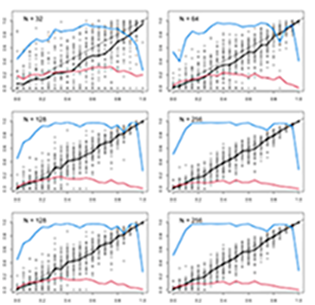
\includegraphics{new.fig.1.temp.png}
\caption{Patterns in \(\lambda\).{}}
\end{figure}

\textbf{Kappa (\(\kappa\)) estimates of phylogenetic signal are more
stable.} Simulation results for \(\kappa\) demonstrated that this
measure displayed better statistical properties. First, as expected,
mean values of \(\kappa\) increased consistently with increasing signal
(\(\lambda\)) irrespective of tree size (Fig. 2 black line).
Additionally, the standard deviation of \(\kappa\) was consistent across
tree sizes (Fig. 2 red line), and while it increased with \(\lambda\),
it was always less than the corresponding mean. This finding is perhaps
unsurprising, as \(\kappa\) is bound by 0, and was never large for small
values of \(\lambda\). Importantly, \(\kappa\) was normally distributed
across the range of input \(\lambda\), and remained consistent in this
pattern regardless of tree size (Fig. 2 blue line). In fact,
distributions of \(\kappa\) displayed slight skewing only at small tree
sizes and when \(\lambda\) was near or equal to \(1\). This result
differs from those of (20), where skewing appears to be from combining
random values generated independently. These findings reveal that
\(\kappa\) is more reliable as an estimate of phylogenetic signal.

\begin{figure}
\centering
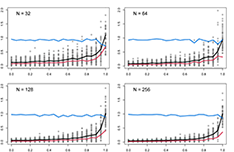
\includegraphics{new.fig.2.temp.png}
\caption{Patterns in \(\kappa\).{}}
\end{figure}

\textbf{Effect sizes from \(\kappa\) (\(Z_{\kappa}\)) better
characterize phylogenetic signal.} To measure the strength of
phylogenetic signal on a common scale, we derived effect sizes
(Z-scores) for both \(\lambda\) and \(\kappa\) (see Methods) and
evaluated them relative to known phylogenetic signal. Both
\(Z_{\lambda}\) and \(Z_{\kappa}\) were associated with input
phylogenetic signal (\(\lambda\)), indicating that both statistics
captured the observed signal (Fig. 3). However, effect sizes from
\(\hat{\lambda}\) made little sense, as they were more strongly
associated with tree size than they were with the actual phylogenetic
signal in the data (Fig. 3). By contrast, \(Z_{\kappa}\) was much more
consistent accross tree sizes, and exhibited a much stronger association
with phylogenetic signal strength as compared to tree size (Fig. 3).
Thus between the two statistics, \(Z_{\kappa}\) is a more reliable
measure of the strength of phylogenetic signal, and may be used to
compare levels of phylogenetic signal across datasets.

\begin{figure}
\centering
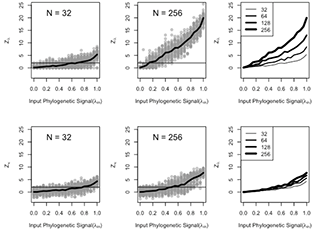
\includegraphics{new.fig.3.temp.png}
\caption{Patterns in Z.{}}
\end{figure}

\textbf{A test statistic (\(\hat{Z}_{12}\)) allows meaningful
comparisons across datasets.} To statistically compare the strength of
phylogenetic signal across datasets we derived a two-sample test
statistic (\(\hat{Z}_{12}\): see Methods). As an example of its utility,
we compared \(Z_{\kappa}\) for two ecologically-relevant traits in
plethodontid salamander (Fig. 4): surface area to volume ratios (SA:V)
and relative body width (\(\frac{BW}{SVL}\)) (33, 34). While both traits
contained significant phylogenetic signal, tests based on
\(\hat{Z}_{12}\) revealed that the degree of phylogenetic signal was
significantly stronger in SA:V (Fig. 4). Biologically, this observation
may be interpreted by the fact that tropical species -- which form a
monophyletic group within plethodontids -- display greater variation in
SA:V, which covaries with disparity in their climatic niches (34). Thus,
greater phylogenetic signal in SA:V is to be expected.

\begin{figure}
\centering
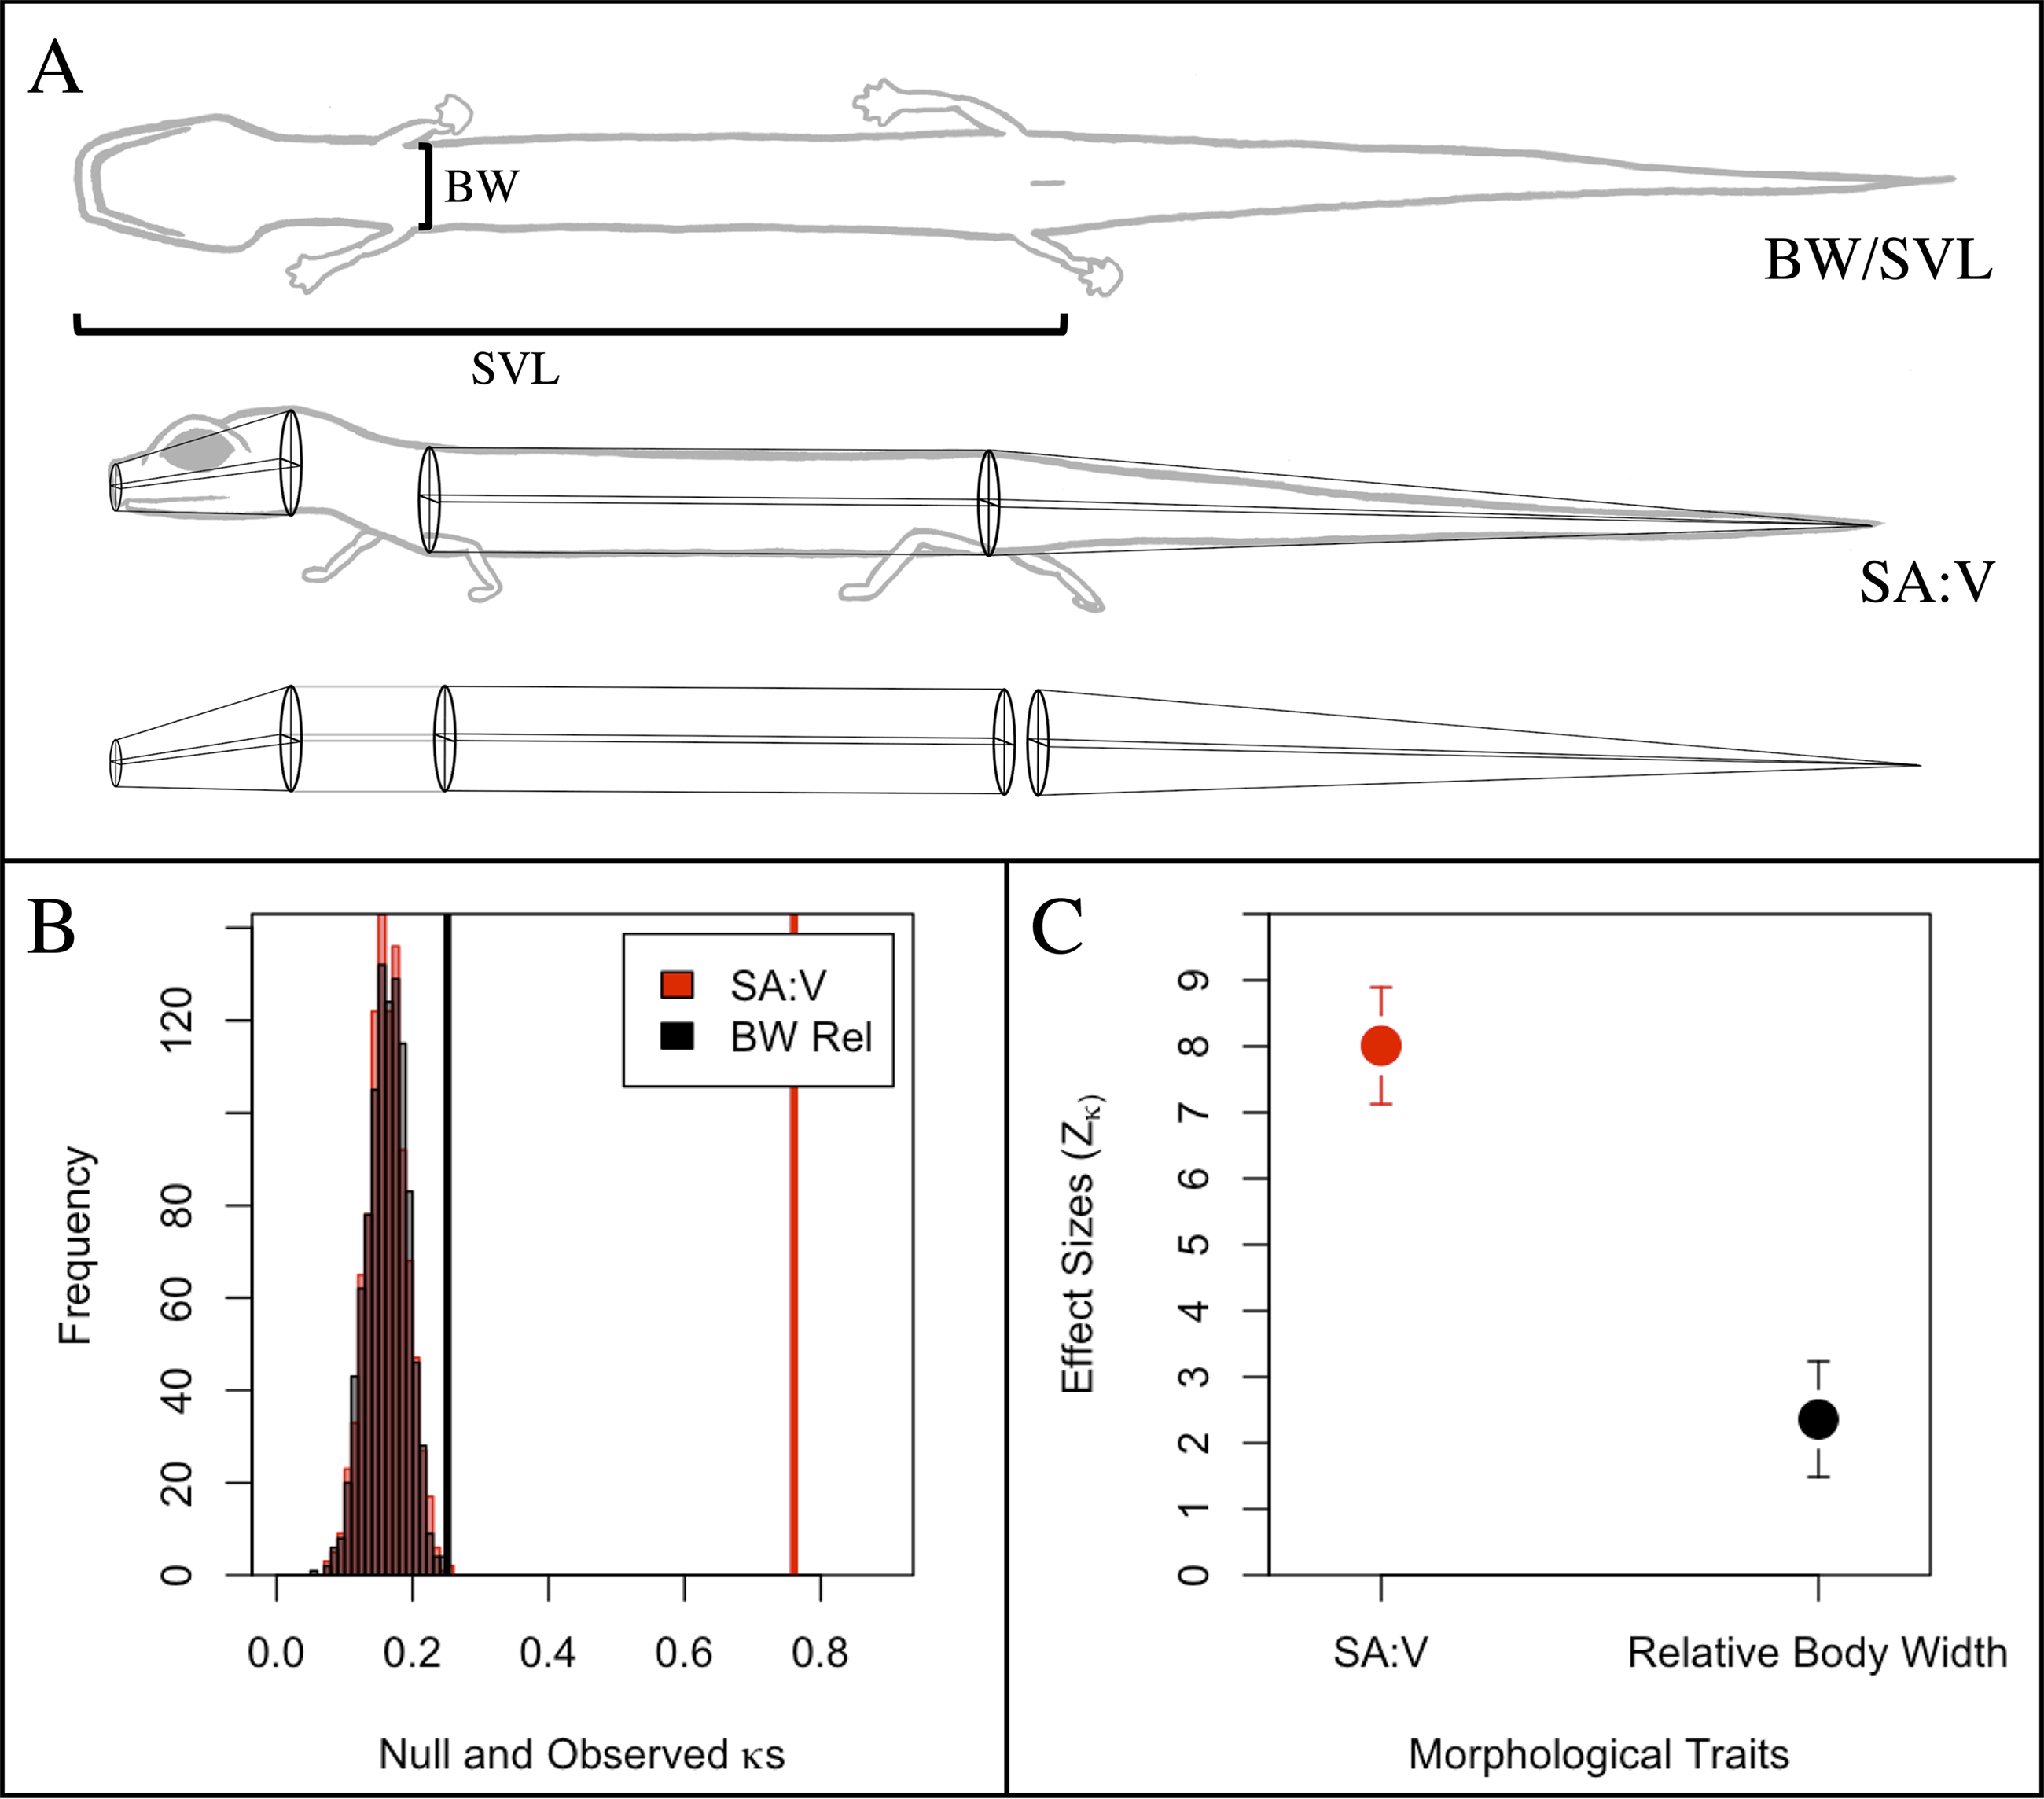
\includegraphics{new.fig.4.png}
\caption{(A) Linear measures for relative body size, and regions of the
body used to estimate surface area to volume (SA:V) ratios. (B)
Permutation distributions of phylogenetic signal for SA:V and
\(\frac{BW}{SVL}\), with observed values shown as vertical bars. (C)
Effect sizes (\(Z_\kappa\)) for SA:V and \(\frac{BW}{SVL}\), with their
95\% confidence intervals (CI not standardized by \(\sqrt(n)\)).{}}
\end{figure}

\hypertarget{discussion}{%
\section{Discussion}\label{discussion}}

\textbf{To be edited.} address hypotheses that compare the strength of
phylogenetic signal between various phenotypic traits, even when those
traits are found in different evolutionary lineages or have different
units or scales.

It is common in comparative evolutionary studies to characterize the
phylogenetic signal in phenotypic traits to determine the extent to
which shared evolutionary history has generated trait covariation among
taxa. However, while numerous analytical approaches may be used to
quantify phylogenetic signal (13, 14, 16--18), methods that explicitly
measure the strength of phylogenetic signal, or facilitate comparisons
among datasets, have remained underdeveloped. In this study, we
evaluated the precision of one common measure, Pagel's \(\lambda\), and
explored its efficacy for characterizing the strength of phylogenetic
signal in phenotypic data. Using computer simulations, we found that the
precision of \(\lambda\) increased with increasing sample sizes; a
pattern noted previously (25), and one that conformed with parametric
statistical theory (35). However, we also found that vastly different
\(\lambda\) estimates could be obtained from data containing the same
level of phylogenetic signal, and that similar \(\lambda\) estimates may
be obtained from data containing differing levels of phylogenetic
signal. Further, the precision of \(\lambda\) varied with the strength
of phylogenetic signal, where lower precision was observed when in data
whose phylogenetic signal was of intemediate strength. From these
findings we conclude that \(\lambda\) is not a reliable indicator of the
observed strength of phylogenetic signal in phenoytpic datasets, and
that biological interpretations of the strength of signal based on this
parameter may innacurately characterize such effects.

As an alternative, we described a standardized effect size (\(Z\)) for
assessing the strength of phylogenetic signal. \(Z\) expresses the
magnitude of phylogenetic signal as a standard normal deviate, which is
easily interpretable as the strength of phylogenetic signal relative to
the mean. We applied this concept to both \(\lambda\) and \(\kappa\),
and found that \(Z_\kappa\) was a better estimate of the strength of
phylogenetic signal in phenotypic data. First, \(Z_\kappa\) was more
precise than \(Z_\lambda\), and precision was more consistent across the
range of input levels of phylogenetic signal. Additionally, values of
\(Z_\kappa\) more accurately tracked known changes in the magnitude of
phylogenetic signal, as demonstrated by the linear relationship between
\(Z_\kappa\) and \(\lambda_{in}\). Thus, \(Z_\kappa\) holds promise as a
measure of the relative strength of phylogenetic signal that reflects
the magnitude of this effect in phenotypic data. We therefore recommend
that future studies interested in the strength of phylogenetic signal
incorporate \(Z_\kappa\) as a statistical measure of this effect.

Based on the effect size \(Z_\kappa\), we then proposed a two-sample
test, which provides means of determining whether the strength of
phylogenetic signal is greater in one phenotypic trait as compared to
another, via a hypothesis test. Prior studies have summarized patterns
of variation in phylogenetic signal across datasets using summary test
values, such as \(\kappa\) (14). However, \(\kappa\) does not scale
linearly with input levels of phylogenetic signal, and its variance
increases (i.e., precision decreases) with increasing strength of
phylogenetic signal (20, 22). Thus, \(\kappa\) should not be considered
an effect size that measures the strength of phylogenetic signal on a
common scale. By contrast, standardizing \(\kappa\) (\(Z_\kappa\), via
equation 2) alleviates these concerns, and facilitates formal
statistical comparisons of the strength of signal across datasets. Thus
when viewed from this perspective, the approach developed here aligns
well with other statistical approaches such as meta-analysis (36--38),
where summary statistics across datasets are converted to standardized
effect sizes for subsequent ``higher order'' statistical summaries or
comparisons. As such, our approach enables evolutionary biologists to
quantitatively examine the relative strength of phylogenetic signal
across a wide range of phenotypic traits, and thus opens the door for
future discoveries that inform on how phenotypic diversity accumulates
in macroevolutionary time across the tree of life.

One important advantage of the approach advocated here is that the
resulting effect sizes (\(Z_\kappa\)) are dimensionless, as the units of
measurement cancel out during the calculation of \(Z\) (39). Thus,
\(Z_\kappa\) represents the strength of phylogenetic signal on a common
and comparable scale -- measured in standard deviations -- regardless of
the initial units and original scale of the phenotypic variables under
investigation. This means that the strength of phylogenetic signal may
be compared across datsets for continuous phenotypic traits measured in
different units and scale, because those units have been standardized
through their conversion to \(Z_\kappa\). For example, our approach
could be utilized to determine whether the strength of phylogenetic
signal (say, in response to ecological differentiation) is stronger in
morphological traits (linear traits: \(mm\)), physiological traits
(metabolic rate: \(\frac{O^2}{min}\)), or behavioral traits (aggression:
\(\frac{\#{displays}}{second}\)). In fact, our empirical example
provided such a comparison, as SA:V is represented in \(mm^{-1}\) while
relative body size is a unitless ratio (\(\frac{BW}{SVL}\)).
Additionally, our method is capable of comparing the strength of
phylogenetic signal in traits of different dimensionality, as estimates
of phylogenetic signal using \(\kappa\) have been generalized for
multivariate data (18). Furthermore, tests based on \(\hat{Z}_{12}\) may
be utilized for comparing the strength of phylogenetic signal among
datasets containing a different number of species, and even for
phenotypes obtained from species in different lineages, because their
phylogenetic non-independence and observed variation are taken into
account in the generation of the empirical sampling distribution via
permutation.

This study is not the first to compare \(\lambda\) and \(\kappa\) for
their ability as statistics to measure phylogenetic signal. Our results
for \(\lambda\) and \(\kappa\) values are consistent with those found in
the simulations performed by Münkemüller et al.~(20), but that study
investigated type I error rates and statistical power, finding that
\(\lambda\) performed better in both regards, irrespective of species
number in trees. Although not the central focus of their study, the same
tendency for variable \(\lambda\) and consistent \(\kappa\) at
intermediate phylogenetic signal strengths was observed (20). Recent
work by Molina-Venegas and Rodríguez (23) found that \(\kappa\) but not
\(\lambda\) tended to inflate the estimate of phylogenetic signal,
leading to moderate type I and type II biases, if polytomic chronograms
were used. Their work more thoroughly addressed previous observations of
inflated \(\kappa\) for incompletely resolved phylogenetic trees (20,
40). An interesting question is whether an inflated \(\kappa\) value
leads to an inflated \(Z_\kappa\) or does a tendency of a particular
tree to inflate estimates of \(\kappa\) also inflate the values in
random permutations of a test, in which case \(Z_\kappa\) is robust to
polytomies? We repeated the analyses in Figure 4, adjusting trees to
have 50\% collapsed nodes, per the technique of Molina-Venegas and
Rodríguez (23), and found results were consistent (see Supporting
Information). This confirms that any tendency of incompletely resolved
trees to inflate \(\kappa\) as a descriptive statistic does not inflate
\(Z_\kappa\) as an effect size. Furthermore, because comparison of
effect sizes in a test is a comparison of locations of observed values
in their sampling distributions, which would shift concomitantly because
of this tendency, the \(Z_{12}\) test statistic in equation 4 appears to
be robust in spite of unresolved trees.

Phylogenetic signal can be thought of as both an attribute to be
measured in the data and a parameter that can be tuned to account for
the phylogenetic non-independence among observations, for analysis of
the data. As such, \(\lambda\) is appealing, as a statistic that
potentially fulfills both roles. However, the inability to estimate
phylogenetic signal with \(\lambda\) for data simulated with known
phylogenetic signal is troublesome, and we recommend evolutionary
biologists refrain from viewing it as a statistic to describe the amount
of phylogenetic signal in the data. Interestingly, \(\kappa\) -- when
standardized to an effect size \(Z_\kappa\) -- is a better statistic for
measuring the amount of phylogenetic signal in data simulated with
respect to known levels of \(\lambda\). Although \(\lambda\) might be
viewed as an important parameter for modifying the the conditional
estimation of linear model coefficients with respect to phylogeny, it is
neither a statistic that has meaningful comparative value as a measure
of phylogenetic signal nor a statistic that lends itself well to
reliable calculation of a test statistic. By contrast, \(\kappa\) has
been shown here to be a reliable statistic, but only when standardized
by the mean and standard deviation of its empirical sampling
distribution (i.e., when converted to the effect size, \(Z_\kappa\)).
Because one has control over the number of permutations used in
analysis, one can be assured with many permutations that the empirical
sampling distribution is representative of true probability
distributions (12). With low coefficients of variation for \(Z_\kappa\)
(Figure 4), it is difficult to imagine that a hypothesis test can
improve equation 4 for efficiently comparing phylogenetic signal for
different traits, different trees, or a combination of both.

\hypertarget{methods}{%
\section{Methods}\label{methods}}

\textbf{Derivation of effect sizes.} Statistically, a standardized
effect size may be found as:

\begin{align}
    Z_{\theta}=\frac{\theta_{obs}-E(\theta)}{\sigma_\theta}
\end{align}

where \(\theta_{obs}\) is the observed test statistic, \(E(\theta)\) is
its expected value under the null hypothesis, and \(\sigma_\theta\) is
its standard error (35, 37, 41). Typically, \(\theta_{obs}\) and
\(\sigma_\theta\) are estimated from the data, while \(E(\theta)\) is
obtained from the distribution of \(\theta\) derived from parametric
theory. However, recent advances in resampling theory (42--45) have
shown that \(E(\theta)\) and \(\sigma_\theta\) may also be obtained from
an empirical sampling distribution of \(\theta\) obtained from
permutation procedures.

Formalizing the suggestion of Adams and Collyer (46), an effect size for
\(\kappa\) may be found as:

\begin{align}
    Z_\kappa=\frac{\kappa_{obs}-\hat\mu_{\kappa}}{\hat\sigma_{\kappa}},
\end{align}

where \(\kappa_{obs}\) is the observed phylogenetic signal, and
\(\hat\mu_\kappa\) and \(\hat\sigma_\kappa\) are the mean and standard
deviation of the empirical sampling distribution of \(\kappa\) obtained
via permutation. The empirical sampling distribution of \(\kappa\) is
first transformed via Box-Cox to better adhere to the assumption of
normality.

For \(\lambda\), deriving an effect size is more challenging, as
\(\lambda\) does not have a sampling distribution from which the
standard error (and thus confidence intervals) may be obtained.
Confidence intervals are tehrefore generated for the values of
\(\lambda\) that intersect the log-likehihood profile for corresponding
percentiles of the \(\chi^2\) distribution used to compare the putative
model to a null model with \(\lambda = 0\) {[}\textbf{add ref: MLC
thinks Boettiger paper?}{]}. Thus, an effect size for \(\lambda\) may be
found as:

\begin{align}
   \lvert Z_{\lambda} \rvert = \sqrt{\chi^2_{\hat{\lambda}}}
\end{align}

where, \(\hat{\lambda}\) is the maximized likelihood value of
\(\lambda\) and \(\chi^{2}_{\hat{\lambda}}\) is the likelihood ratio
statistic for the value. Note that alternative formulations could be
envisioned: \(Z_{\lambda} = d \sqrt{\chi^2_{\hat{\lambda}}}\), where
\(d\) is a binary value \((-1,1)\) to indicate a direction based on
whether \(\hat{\lambda}\) is below or above a critical value of
\(\lambda\), for a quantile from a \(\chi^{2}\) distribution at a
probability of 0.5. However, preliminary investigations found that
mapping \(\chi^2_{\hat{\lambda}}\) values in this manner did not produce
effect sizes that were symmetrical about \(Z = 0\), as the mapping was
not linear and the log-likelihood profiles can be rather flat for small
trees. \textbf{Is alternative needed here?}

\textbf{Derivation of two-sample test statistic.} To compare the
strength of phylogenetic signal across datasets, a two-sample test
statistic may be calculated as:

\begin{align}
  \hat{Z}_{12}=\frac{\lvert{(\kappa_{1}-\hat\mu_{\kappa_1})-(\kappa_{2}-\hat\mu_{\kappa_2})}\rvert}{\sqrt{\hat\sigma^2_{\kappa_1}+\hat\sigma^2_{\kappa_2}}} = \frac{\lvert Z_{\kappa_1} - Z_{\kappa_2}\rvert}{\sqrt{2}}
\end{align}

where \(\kappa_1\), \(\kappa_2\), \(\hat\mu_{\kappa_1}\),
\(\hat\mu_{\kappa_2}\), \(\hat\sigma_{\kappa_1}\), and
\(\hat\sigma_{\kappa_2}\) are as defined above for equation 2. The right
side of the equation illustrates that if \(Z_\kappa\) has already been
calculated for two sampling distributions as in equation 2, the sampling
distributions have unit variance for each of the \(Z_\kappa\)
statistics. Estimates of significance of \(\hat{Z}_{12}\) may be
obtained from a standard normal distribution. Typically,
\(\hat{Z}_{12}\) is considered a two-tailed test, however directional
(one-tailed) tests may be specified should the empirical situation
require it (43, 45).

\textbf{Simulations.} Simulations were conducted by generating
pure-birth phylogenies at each of six different tree sizes
(\(n=2^5, 2^6, \cdots, 2^{10}\)), and with differing levels of
phylognetic signal (\(\lambda=0.0, 0.5, \cdots, 1.0\)). We generated 100
random trees for each intersection of tree size and \(\lambda\). For
each \(\lambda\) within each tree size, continuous traits were then
simulated on each phylogeny under a BM model of evolution. For each set
of 100 trees we measured the mean values of \(\hat{\lambda}\) and
\(\kappa\), their standard deviation, and calculated the Shapiro-Wilk
\(W\) statistic as a departure from normality (symmetry). For the
latter, a value of \(1.0\) indicates normally distributed values, while
departures from \(1.0\) indicate skewness. Simulations were then
repeated for both bananced and pectinate trees, which yielded
qualitatively similar results (see Supporting Information). Trees
containing polytomies, and an evaluation of \(\hat{\lambda}\) from
models of linear regression and phylogenetic ANOVA, were also
investigated, and results were qualitatively similar to those reported
above (see Supporting Information).

\textbf{Empirical Data.} Surface area to volume ratios (SA:V) and
relative body width (\(\frac{BW}{SVL}\)) measures were obtained from as
species means from individuals of 305 species, from which species means
were obtained (33, 34). A time-dated molecular phylogeny for the group
(47) was pruned to match the species in the phenotypic dataset. The
phylogenetic signal in each trait was then characterized using
\(\kappa\), which was converted to its effect size (\(Z_\kappa\)) using
\texttt{geomorph} 3.3.1 (48, 49), and routines by the authors
(\textbf{to be incorporated in \texttt{geomorph} upon manuscript
acceptance}).

\showmatmethods
\showacknow
\pnasbreak

\hypertarget{refs}{}
\leavevmode\hypertarget{ref-Felsenstein1985}{}%
1. Felsenstein J (1985) Phylogenies and the comparative method.
\emph{American Naturalist} 125(1):1--15.

\leavevmode\hypertarget{ref-HarveyPagel1991}{}%
2. Harvey PH, Pagel MD (1991) \emph{The comparative method in
evolutionary biology} (Oxford University Press, Oxford).

\leavevmode\hypertarget{ref-Grafen1989}{}%
3. Grafen A (1989) The phylogenetic regression. \emph{Philosophical
Transactions of the Royal Society of London B, Biological Sciences}
326:119--157.

\leavevmode\hypertarget{ref-GarlandIves2000}{}%
4. Garland TJ, Ives AR (2000) Using the past to predict the present:
Confidence intervals for regression equations in phylogenetic
comparative methods. \emph{American Naturalist} 155:346--364.

\leavevmode\hypertarget{ref-Rohlf2001}{}%
5. Rohlf FJ (2001) Comparative methods for the analysis of continuous
variables: Geometric interpretations. \emph{Evolution} 55:2143--2160.

\leavevmode\hypertarget{ref-ButlerKing2004}{}%
6. Butler MA, King AA (2004) Phylogenetic comparative analysis: A
modeling approach for adaptive evolution. \emph{American Naturalist}
164:683--695.

\leavevmode\hypertarget{ref-MartinsHansen1997}{}%
7. Martins EP, Hansen TF (1997) Phylogenies and the comparative method:
A general approach to incorporating phylogenetic information into the
analysis of interspecific data. \emph{American Naturalist} 149:646--667.

\leavevmode\hypertarget{ref-OMeara_et_al2006}{}%
8. O'Meara BC, Ane C, Sanderson MJ, Wainwright PC (2006) Testing for
different rates of continuous trait evolution using likelihood.
\emph{Evolution} 60:922--933.

\leavevmode\hypertarget{ref-RevellHarmon2008}{}%
9. Revell LJ, Harmon LJ (2008) Testing quantitative genetic hypotheses
about the evolutionary rate matrix for continuous characters.
\emph{Evolutionary Ecology Research} 10:311--331.

\leavevmode\hypertarget{ref-Beaulieu_et_al2012}{}%
10. Beaulieu JM, Jhwueng DC, Boettiger C, O'Meara BC (2012) Modeling
stabilizing selection: Expanding the ornstein-uhlenbeck model of
adaptive evolution. \emph{Evolution} 66:2369--2383.

\leavevmode\hypertarget{ref-Adams2014b}{}%
11. Adams DC (2014) A method for assessing phylogenetic least squares
models for shape and other high-dimensional multivariate data.
\emph{Evolution} 68:2675--2688.

\leavevmode\hypertarget{ref-AdamsCollyer2018b}{}%
12. Adams DC, Collyer ML (2018) Phylogenetic anova: Group-clade
aggregation, biological challenges, and a refined permutation procedure.
\emph{Evolution} 72(6):1204--1215.

\leavevmode\hypertarget{ref-Pagel1999}{}%
13. Pagel MD (1999) Inferring the historical patterns of biological
evolution. \emph{Nature} 401:877--884.

\leavevmode\hypertarget{ref-Blomberg_et_al2003}{}%
14. Blomberg SP, Garland T, Ives AR (2003) Testing for phylogenetic
signal in comparative data: Behavioral traits are more labile.
\emph{Evolution} 57:717--745.

\leavevmode\hypertarget{ref-Revell_et_al2008}{}%
15. Revell LJ, Harmon LJ, Collar DC (2008) Phylogenetic signal,
evolutionary process, and rate. \emph{Systematic Biology} 57:591--601.

\leavevmode\hypertarget{ref-Abouheif1999}{}%
16. Abouheif E (1999) A method for testing the assumption of
phylogenetic independence in comparative data. \emph{Evolutionary
Ecology Research} 1:895--909.

\leavevmode\hypertarget{ref-Gittleman1990}{}%
17. Gittleman JL, Kot M (1990) Adaptation: Statistics and a null model
for estimating phylogenetic effects. \emph{Systematic Zoology}
39(3):227--241.

\leavevmode\hypertarget{ref-Adams2014a}{}%
18. Adams DC (2014) A generalized Kappa statistic for estimating
phylogenetic signal from shape and other high-dimensional dultivariate
data. \emph{Systematic Biology} 63:685--697.

\leavevmode\hypertarget{ref-Klingenberg2010}{}%
19. Klingenberg CP, Gidaszewski NA (2010) Testing and quantifying
phylogenetic signals and homoplasy in morphometric data.
\emph{Systematic biology} 59(3):245--261.

\leavevmode\hypertarget{ref-Munkemuller_et_al2012}{}%
20. Münkemüller T, et al. (2012) How to measure and test phylogenetic
signal. \emph{Methods in Ecology and Evolution} 3:743--756.

\leavevmode\hypertarget{ref-Pavoine2012}{}%
21. Pavoine S, Ricotta C (2012) Testing for phylogenetic signal in
biological traits: The ubiquity of cross-product statistics.
\emph{Evolution: International Journal of Organic Evolution}
67(3):828--840.

\leavevmode\hypertarget{ref-DinizFilho2012}{}%
22. Diniz-Filho JAF, Santos T, Rangel TF, Bini LM (2012) A comparison of
metrics for estimating phylogenetic signal under alternative
evolutionary models. \emph{Genetics and Molecular Biology}
35(3):673--679.

\leavevmode\hypertarget{ref-MolinaVenegas2017}{}%
23. Molina-Venegas R, Rodríguez MA (2017) Revisiting phylogenetic
signal; strong or negligible impacts of polytomies and branch length
information? \emph{BMC evolutionary biology} 17(1):53.

\leavevmode\hypertarget{ref-Revell2010}{}%
24. Revell LJ (2010) Phylogenetic signal and linear regression on
species data. \emph{Methods in Ecology and Evolution} 1:319--329.

\leavevmode\hypertarget{ref-Boettiger_et_al2012}{}%
25. Boettiger C, Coop G, Ralph P (2012) Is your phylogeny informative?
Measuring the power of comparative methods. \emph{Evolution}
67:2240--2251.

\leavevmode\hypertarget{ref-Freckleton_et_al2002}{}%
26. Freckleton RP, Harvey PH, Pagel M (2002) Phylogenetic analysis and
comparative data: A test and review of evidence. \emph{American
Naturalist} 160:712--726.

\leavevmode\hypertarget{ref-Cooper2010}{}%
27. Cooper N, Jetz W, Freckleton RP (2010) Phylogenetic comparative
approaches for studying niche conservatism. \emph{Journal of
Evolutionary Biology} 23(12):2529--2539.

\leavevmode\hypertarget{ref-Bose2019}{}%
28. Bose R, Ramesh BR, Pélissier R, Munoz F (2019) Phylogenetic
diversity in the western ghats biodiversity hotspot reflects
environmental filtering and past niche diversification of trees.
\emph{Journal of Biogeography} 46(1):145--157.

\leavevmode\hypertarget{ref-Vandelook2019}{}%
29. Vandelook F, et al. (2019) Nectar traits differ between pollination
syndromes in balsaminaceae. \emph{Annals of Botany} 124(2):269--279.

\leavevmode\hypertarget{ref-DeMeester2019}{}%
30. De Meester G, Huyghe K, Van Damme R (2019) Brain size, ecology and
sociality: A reptilian perspective. \emph{Biological Journal of the
Linnean Society} 126(3):381--391.

\leavevmode\hypertarget{ref-Pintanel2019}{}%
31. Pintanel P, Tejedo M, Ron SR, Llorente GA, Merino-Viteri A (2019)
Elevational and microclimatic drivers of thermal tolerance in andean
pristimantis frogs. \emph{Journal of Biogeography} 46(8):1664--1675.

\leavevmode\hypertarget{ref-Su2019}{}%
32. Su G, Villéger S, Brosse S (2019) Morphological diversity of
freshwater fishes differs between realms, but morphologically extreme
species are widespread. \emph{Global ecology and biogeography}
28(2):211--221.

\leavevmode\hypertarget{ref-Baken2019}{}%
33. Baken EK, Adams DC (2019) Macroevolution of arboreality in
salamanders. \emph{Ecology and Evolution} 9(12):7005--7016.

\leavevmode\hypertarget{ref-Baken2020}{}%
34. Baken EK, Mellenthin LE, Adams DC (2020) Macroevolution of
desiccation‐related morphology in plethodontid salamanders as inferred
from a novel surface area to volume ratio estimation approach.
\emph{Evolution} 74:476--486.

\leavevmode\hypertarget{ref-Cohen1988}{}%
35. Cohen J (1988) \emph{Statistical power analysis for the behavioral
sciences} (Routledge).

\leavevmode\hypertarget{ref-HedgesOlkin1985}{}%
36. Hedges L. V., Olkin I (1985) \emph{Statistical methods for
meta-analysis} (Elsevier).

\leavevmode\hypertarget{ref-Glass1976}{}%
37. Glass GV (1976) Primary, secondary, and meta-analysis of research.
\emph{Educational Researcher} 5:3--8.

\leavevmode\hypertarget{ref-Arnqvist1995}{}%
38. Arnqvist G., Wooster D (1995) Meta-analysis: Synthesizing research
findings in ecology and evolution. \emph{Trends in Ecology and
Evolution} 10:236--240.

\leavevmode\hypertarget{ref-SokalRohlf2012}{}%
39. Sokal R. R., Rohlf FJ (2012) \emph{Biometry} (W.H. Freeman \& Co.,
San Francisco). 4th Ed.

\leavevmode\hypertarget{ref-Davies2012}{}%
40. Davies TJ, Kraft NJ, Salamin N, Wolkovich EM (2012) Incompletely
resolved phylogenetic trees inflate estimates of phylogenetic
conservatism. \emph{Ecology} 93(2):242--247.

\leavevmode\hypertarget{ref-Rosenthal1994}{}%
41. Rosenthal R (1994) The handbook of research synthesis. ed Cooper LV
H Hedges (Russell Sage Foundation), pp 231--244.

\leavevmode\hypertarget{ref-Collyer_et_al2015a}{}%
42. Collyer ML, Sekora DJ, Adams DC (2015) A method for analysis of
phenotypic change for phenotypes described by high-dimensional data.
\emph{Heredity} 115:357--365.

\leavevmode\hypertarget{ref-AdamsCollyer2016}{}%
43. Adams DC, Collyer ML (2016) On the comparison of the strength of
morphological integration across morphometric datasets. \emph{Evolution}
70:2623--2631.

\leavevmode\hypertarget{ref-CollyerAdams2018}{}%
44. Collyer ML, Adams DC (2018) RRPP: An r package for fitting linear
models to high-dimensional data using residual randomization.
\emph{Methods in Ecology and Evolution} 9:1772--1779.

\leavevmode\hypertarget{ref-AdamsCollyer2019b}{}%
45. Adams DC, Collyer ML (2019) Comparing the strength of modular
signal, and evaluating alternative modular hypotheses, using covariance
ratio effect sizes with morphometric data. \emph{Evolution}
73(12):2352--2367.

\leavevmode\hypertarget{ref-AdamsCollyer2019}{}%
46. Adams DC, Collyer ML (2019) Phylogenetic comparative methods and the
evolution of multivariate phenotypes. \emph{Annual Review of Ecology,
Evolution, and Systematics} 50:405--425.

\leavevmode\hypertarget{ref-Bonett2017}{}%
47. Bonett RM, Blair AL (2017) Evidence for complex life cycle
constraints on salamander body form diversification. \emph{Proceedings
of the National Academy of Sciences, USA} 114:9936--9941.

\leavevmode\hypertarget{ref-AdamsOtarola2013}{}%
48. Adams DC, Otárola-Castillo E (2013) Geomorph: An r package for the
collection and analysis of geometric morphometric shape data.
\emph{Methods in Ecology and Evolution} 4:393--399.

\leavevmode\hypertarget{ref-AdamsGeomorph}{}%
49. Adams DC, Collyer ML, Kaliontzopoulou A (2020) Geomorph: Software
for geometric morphometric analyses. R package version 3.3.1. Available
at: \url{https://cran.r-project.org/package=geomorph}.



% Bibliography
% \bibliography{pnas-sample}

\end{document}

